\documentclass[../competing_bandits_with_appendix.tex]{subfiles}
\begin{document}

\section{Introduction}\label{section:1}

Many modern online platforms simultaneously compete for users as well as learn from the users they manage to attract. This creates a tradeoff between \textit{exploration} and \textit{competition}: firms experiment with potentially sub-optimal options for the sake of gaining information to make better decisions tomorrow, while they need to incentivize consumers to select them over their competitors today. For instance, Google Search and Bing compete for users in the search engine market yet at the same time need to experiment with their search and ranking algorithms to learn what works best.

Platforms routinely deploy A/B tests, and are increasingly adopting  more sophisticated exploration methodologies based on \emph{multi-armed bandits}, a well-known framework for exploration and making decisions under uncertainty. While deploying ``better" learning algorithms for exploration would improve performance, this is not necessarily beneficial under competition, even putting aside the deployment/maintenance costs. In particular, excessive experimentation may hurt platform's reputation and decrease market share in the near term. This would leave the learning algorithms with less users to learn from, which may further degrade platform's performance relative to competitors who keep learning and improving from \emph{their} users, and so forth.

\gaedit{We ask whether algorithms that are traditionally considered ``better" in the standard multi-armed bandit problem are incentivized to be deployed under competition.} We investigate this issue via extensive numerical experiments in a stylized duopoly model. In our model, two firms compete for users and simultaneously learn from them. Each firm commits to a multi-armed bandit algorithm, and \emph{explores} according to this algorithm. Users select between the two firms based on the current reputation score: rewards from the firm's algorithm, averaged over a recent time window. Each firm's objective is to maximize its \gaedit{expected} market share (the fraction of users choosing this firm).

\tikzstyle{level 1}=[level distance=3.5cm, sibling distance=4.0cm]
\tikzstyle{level 2}=[level distance=3.5cm, sibling distance=2cm]
\tikzstyle{below} = [align=center]

\begin{figure}
\begin{center}
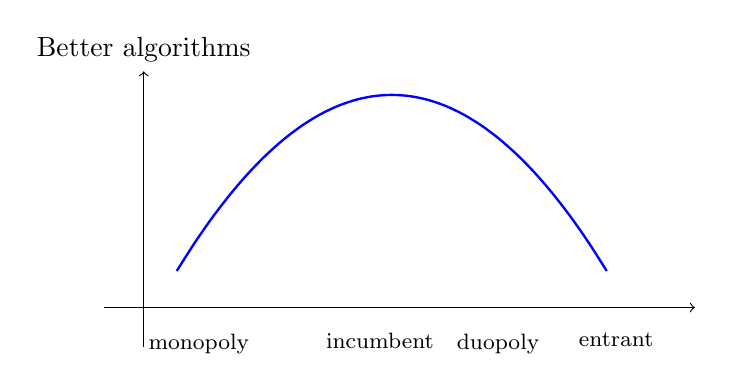
\begin{tikzpicture}
      \draw[->] (-.5,0) -- (7,0) node[right] {};
      \draw[->] (0,-.5) -- (0,3) node[above] {Better algorithms};
      \draw[scale=0.6,domain=0.7:9.8,smooth,variable=\x,blue, line width=0.3mm] plot ({\x},{4.5 - 0.18 * (\x - 5.25)^2});
     \node[below] at (0.7, -0.22) {\footnotesize monopoly};
     \node[below] at (3, -0.2) {\footnotesize incumbent};
     \node[below] at (4.5, -0.22) {\footnotesize duopoly};
     \node[below] at (6, -0.2) {\footnotesize entrant};
 \end{tikzpicture}
 \caption{A stylized ``inverted-U relationship" between strength of competition and ``level of innovation".}
\label{fig:inverted-U}
\end{center}
\end{figure}

We consider a \emph{permanent duopoly} in which both firms start at the same time, as well as \emph{temporary monopoly}: a duopoly with a \gaedit{first-mover}. \swcomment{confused about how they correspond to ``competition intensity''}Accordingly, the intensity of competition in the model varies from ``permanent monopoly" (just one firm) to ``\gadelete{early entry}\gaedit{incumbent}" (the first-mover in temporary monopoly) to permanent duopoly to ``\gadelete{late entry}\gaedit{entrant" (late-arriver in temporary monopoly)}. \gaedit{We find that, even in the permanent duopoly, in equilibrium competition incentivizes firms to play a ``greedy algorithm" that does not explicitly explore and even more so if the firm is a late arriver in a market.} This algorithm also prevails under monopoly, simply because it tends to be easier to deploy. \gaedit{Whereas the incumbent in the temporary monopoly is incentivized to deploy a more advanced exploration algorithm that perform better in the long run. As a result, we find that consumer welfare is highest under temporary monopoly and that even increasing the number of firms in the market past a duopoly makes consumers weakly worse off.}

Interpreting the adoption of better algorithms as ``innovation", our findings can be framed in terms of an ``inverted-U relationship" between competition and innovation (see Figure~\ref{fig:inverted-U}). This relationship -- too little or too much competition is bad for innovation, but intermediate levels of competition tend to be better -- is a familiar theme in the economics literature, dating back to \cite{Schumpeter-42}. \swedit{However, the ``inverted-U relationship'' is driven by different aspects in our model than the ones in the existing literature in economics. In our case, the barriers for innovations arise entirely from the reputational consequences of exploration in competition, as opposed to the R\&D costs (which is the more standard cause in prior work)}.

\gaedit{The findings on temporary monopoly shed light on the ``first-mover advantage" phenomenon in the digital economy. Being first in the market in the digital economy gives firms free data to learn from (a ``data advantage") as well as a more definite, and possibly better reputation compared to an entrant (a ``reputation advantage"). 

\swedit{Beyond the welfare implications, we also investigate the barrier to entry that follows from the incumbent's data advantage.  We run additional experiments that attempt to isolate the impact of the data advantage and reputation advantage. We find that the data advantage from the incumbent's ``small head start'' can lead to a significant incumbency advantage, especially when the incumbent commits to a more advanced bandit algorithm. Our results show that even a small degree of data asymmetry can be amplified to be a larger market advantage through competition dynamics. This is in contrast to the data advantage in a static environment such as discussed in \cite{varian2018artificial,bajari2018impact}, in which a small amount of additional data can only provide limited improvement in the predictive accuracy. 
Our results shed lights on the importance of considering competition dynamics when reasoning about the anti-trust question of whether data can become a significant barrier to entry in an industry. 
% in a competitive environment the relative differences in the data
% possessed by the firms may lead to a large competitive benefit due
% to the feedback loops discussed previously. In our model this effect
% is amplified when the incumbent commits to a more advanced bandit
% algorithm since, in the incumbency period, the firm gathers data on
% possible actions more efficiently leading to the relative gap upon
% entry to be larger. This is important when exploration can have
% larger reputational consequences.
}}\swcomment{still not super happy about above.}

\OMIT{Our findings on temporary monopoly shed light on the ``first-mover advantage" phenomenon in the digital economy. Being first in the market gives firms free data to learn from (a ``data advantage") as well as a more definite, and possibly better reputation compared to an entrant (a ``reputation advantage"). We investigate which of the two is a stronger barrier to entry. We find that both are strong barriers on their own: removing either one still gives the incumbent a substantially larger share of the market compared to the case where both are removed. However, the data advantage tends to be a stronger barrier when the incumbent commits to a more advanced bandit algorithm. One take-away is that the data advantage is not just about data quantity but also data quality.}

We also investigate how algorithms' performance ``in isolation" (without competition) is predictive of the outcomes under competition. In particular, we find that mean reputation -- arguably, the most natural performance measure ``in isolation" -- is sometimes not a good predictor. We suggest a more refined performance measure, and use it to explain (and frame) some of the competition outcomes.


\subsubsection{Related work.}
Our work is related to a longstanding economics literature on competition vs. innovation, \eg \cite{Schumpeter-42,barro2004economic,Aghion-QJE05}. While this literature focuses on R\&D costs of innovation, ``reputational costs" seem new and specific to exploration.

Multi-armed bandits (MAB) is a tractable abstraction for the tradeoff between exploration and \emph{exploitation} (making good near-term decisions based on available information). MAB problems have been studied for many decades, see \cite{Bubeck-survey12} for background. We consider i.i.d. rewards, a well-studied and well-understood MAB model \cite{bandits-ucb1}. We focus on a well-known distinction between ``greedy" (exploitation-only) algorithms, ``naive" algorithms that separate exploration and exploitation, and ``smart" algorithms that combine them. Switching from ``greedy" to ``naive" to ``smart" algorithms involves substantial adoption costs in infrastructure and personnel training \cite{MWT-WhitePaper-2016,DS-arxiv}.

The study of competition vs. exploration has been initiated in \cite{CompetingBandits-itcs16}. Their model differs from ours in two key respects. First, users do not see any signal about firms' past performance, and instead choose between firms according to the Bayesian-expected reward. Second, they vary the strength of competition using assumptions about (ir)rational consumer behavior, whereas we use early entry. Their results are purely theoretical; their model is amenable to proofs but not to numerical experiments. Their high-level conclusion is an inverted-U relationship between competition and innovation that is similar to ours.

The interplay between exploration, exploitation and incentives has been studied in other scenarios: incentivizing exploration in a recommendation system,
    \eg \cite{Kremer-JPE14,Frazier-ec14,Che-13,ICexploration-ec15,Bimpikis-exploration-ms17},
dynamic auctions
    (see \cite{DynAuctions-survey10} for background),
online ad auctions, \eg
    \cite{MechMAB-ec09,DevanurK09,NSV08,Transform-ec10-jacm,Amin-auctions-nips13},
and human computation
    \cite{RepeatedPA-ec14,Ghosh-itcs13,Krause-www13}.
Our setting is also closely related to the ``dueling algorithms" framework \cite{DuelingAlgs-stoc11}, but this framework considers offline / full feedback scenarios whereas we focus on online machine learning problems.
\swedit{There is also a line of work on ``dueling bandits" (e.g., \cite{Yue-dueling-icml09, Yue-dueling12}) that also studies a form of competition with MAB problems. However, their framework is fundamentally different from ours in that they study learning from setting up ``duels'' between pairs of arms, and we study how learning algorithms compete with each other for data.
}

The study of whether data can give a significant \swdelete{competitive} advantage
has been discussed theoretically in \cite{varian2018artificial,
  lambrecht2015can} and empirically in
\cite{bajari2018impact}. \swedit{While they argue that small amounts
  of additional data do not provide significant improvement in
  training a more predictive model, this set of results focus on learning in isolation, which overlooks certain aspects in a competition.
\swdelete{
These studies consider the effect of additional data in terms of helping towards solving a machine learning problem in isolation and argue that it does not play a large role.} We ask how additional data helps while firms simultaneously solve a machine learning problem and compete for consumers. In our setting, the competition dynamics from our model lead to different conclusions about the competitive advantage that a data advantage can give a firm. Additionally, the first-mover advantage has been well-studied in economics and marketing \cite{kerin1992first}. }


\end{document} 
%%% Local Variables:
%%% mode: latex
%%% TeX-master: "../competing_bandits"
%%% End:
